
\documentclass{UoYCSproject}

\addbibresource{Report.bib}
\usepackage{enumerate}
\newcommand\independent{\protect\mathpalette{\protect\independenT}{\perp}}
\def\independenT#1#2{\mathrel{\rlap{$#1#2$}\mkern2mu{#1#2}}}
\usepackage{tikz}
\usepackage{pgflibraryarrows}
\usepackage{multirow}
\usepackage{longtable}
\usepackage[ruled,vlined]{algorithm2e}

\begin{document}
\acknowledgements{I would like to express my gratitude to my supervisor James Cussens for guiding me throughout this project with advice that was crucial to its completion.}
\pagenumbering{roman}
\title{Learning Causal Networks in Python}
\author{James Callan}
\supervisor{James Cussens}
\MEng
\date{}

\maketitle

\listoffigures
\listoftables

\begin{summary}
	The aim of this project was to implement a number of constraint based algorithms for learning causal networks in Python. Three algorithms were considered for implementation, the PC algorithm ~\parencite{spirtes1991algorithm}, the FCI algorithm ~\parencite{colombo2012learning}, and the RFCI algorithm ~\parencite{colombo2012learning}. However due to time constraints only the FCI and the PC algorithms were implemented. These algorithms take data and attempt to infer the causal links between variables based on a series of constraints.
	
	Another aim was to make a code base that could be extended to other algorithms or variations of the implemented algorithms.    
	
	The algorithms had already been implemented in R ~\parencite{kalisch_hauser_maechler}. However due to the growing popularity of machine learning in Python and the wider usage of Python code than R code implementations of these algorithms could be very useful. For example a Python implementation could more easily be integrated into a wider system and work alongside existing Python code.
	
	The Agile methodology was chosen to design and develop the software. This consisted of the project being broken down into a number of ''sprints'' which each implemented a deliverable piece of software. This allowed the project to easily grow as time went on and ensure that working software will be created.  In each sprint requirements were specified, architecture was designed, tests were written and then software was written.
	
	Test driven development was also used, this entailed specifying the functionality of the code with unit tests before implementation and then writing code which could pass these tests. If the tests adequately capture the specified functionality then so will the software.
	
	This project culminated in two of the algorithms being implemented, the PC and FCI algorithms, along with a $\chi^2$ test for conditional independence. Comparisons of the Python implementation to the R implementation found issues of order dependence in the algorithms. There is no particular order in which to search networks for edges for each particular orientation rule. This leads to two implementations which correctly implement the algorithms producing different results. These issues have been addressed in modified versions of the algorithms ~\parencite{colombo2014order}, some of which have been implemented in the R implementation. The time constraints of this project unfortunately made these modified algorithms unfeasible to implement, however they are obvious candidates for future work on this project.
	
	Testing based on the R implementation along with testing based on the known behaviour of the algorithm on simple networks was used to validate the software and prove that it is a correct implementation of the described algorithms.
	
	The Python code was also found to run significantly slower than the R implementation. This was mostly due to the $\chi^2$ test for independence which was using a built in function of the pandas library which is very slow.
	
	The main issues with this project would occur if it were to be distributed. Many open source python libraries and datasets were used to develop this software, the licensing agreements of this content must be followed. Copyright law would have to be considered and the copyright of the open source projects and datasets utilised respected.
	
	There are few ethical issues in this project, the project is highly unlikely to be used in safety critical applications. However any user of this software should be aware that the networks generated by this software may be inaccurate. Unlike other methods the algorithms implemented do not produce a measure of confidence in the accuracy of the graph.
	
	
\end{summary}
\chapter{Introduction}
The aim of this report is to detail the implementation of various algorithms to learn causal networks in Python (the PC ~\parencite{spirtes1991algorithm}, FCI ~\parencite{colombo2012learning}, and RFCI ~\parencite{colombo2012learning} algorithms). These algorithms have already been implemented in the statistical programming language R ~\parencite{kalisch_hauser_maechler}. However, recently python has become more widely used in the field of statistical computation and machine learning ~\parencite{piatetsky}.

Python offers a number of advantages over R. Python is much more widely used in general than R ~\parencite{ogrady_2019} so an implementation in Python would be accessible to a wider array of developers. Python can also be used in a wider variety of settings than R. R is designed for data analysis and data visualisation, whereas Python is designed to be general purpose. This makes it easier in Python than in R to incorporate data analysis into wider systems such as websites or desktop applications.

These algorithms could be useful in a number of situations. They could be useful for data scientists attempting to find the cause of a particular variable. They could also aid in basic data exploration, showing the dependencies which can be exploited for further analysis in a human readable fashion. 

This project should also produce a codebase that is easy to extend to incorporate more network learning algorithms. Data structures which can be used by other algorithms not in the scope of this project should be made to be easy to use and extensible.

\chapter{Literature Review}

\section{Causal Networks}

Causal Networks are graphical models which represent a set of variables, their conditional dependencies, and their causal relationships~\parencite{verma1990causal} as a Directed Acyclic Graph (DAG) in Figure 2.1 or a Maximal Ancestral Graph (MAG) in Figure 2.2. The nodes of the Graph represent the variables. The edges of the graph represent causality, the direction of the edge represents the direction of causality with parent nodes causing child nodes~\parencite{verma1990causal}. 

In a DAG all edges have a single direction, whereas in a MAG edges may be directed or bidirectional ~\parencite{zhang2008causal}.

\begin{figure}[h]
	\begin{center}		
	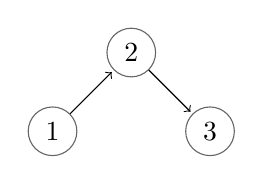
\begin{tikzpicture}[shorten >=1pt,->]
	\tikzstyle{vertex}=[circle, draw=black!60, minimum size=12pt]
	\node[vertex] (G_1) at (-1,-1) {1};
	\node[vertex] (G_2) at (0,0)   {2};
	\node[vertex] (G_3) at (1,-1)  {3};
	\draw [->] (G_1) -- (G_2);
	\draw [->] (G_2) -- (G_3);
	\end{tikzpicture}
\end{center}
\caption{A DAG with 3 nodes and 2 edges}
\end{figure}


\begin{figure}[h]
	\begin{center}	
	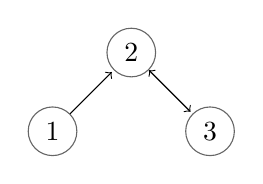
\begin{tikzpicture}[shorten >=1pt,->]
	\tikzstyle{vertex}=[circle, draw=black!60, minimum size=12pt]
	\node[vertex] (G_1) at (4,-1) {1};
	\node[vertex] (G_2) at (5,0)   {2};
	\node[vertex] (G_3) at (6,-1)  {3};
	\draw [->] (G_1) -- (G_2);
	\draw [<->] (G_2) -- (G_3);
	\end{tikzpicture}\\
\end{center}
	\caption{A PDAG with 3 nodes and 2 edges}
\end{figure}



The learning of causal networks allows relationships between variables to be uncovered and presented in a simple and human readable fashion. This can provide useful information for further data analysis as the set of variables which cause another could be used to predict its value. Causal relationships between any pair of variables of a causal network can be easily found. The networks also represent dependencies between variables.

\section{Probability and Independence}

\subsection{Basic Probability}
In probability theory the confidence that a particular event $ E $ occurs can be quantified. This confidence, denoted as $ p(E) $ is a real number between 1 and 0. $  p(E) = 1 $ representing a certainty and $  p(E) = 0 $ representing $E$ being impossible ~\parencite{barber_2012}.

In the case of discrete random variables, an event would be a variable $X$ taking a particular value $x_i$, where $x_i$ is a member of the set $x = \{x_1, x_2, ..., x_n\}$ of possible values that $X$ can take. The probability of this event is denoted as $p(X=x_i)$ ~\parencite{barber_2012}.

\subsection{Distributions}
The probability distribution $p(X=x)$ or simply $p(X)$ defines the likelihood of $X$ taking any value. Distributions can be continuous or discrete depending on the variable ~\parencite{barber_2012}.

Distributions of more than one variable can be described with joint distributions. For variables $X$ and $Y$ the distribution $p(X,Y)$  describes the probability of both $X$ and $Y$ taking particular values simultaneously or $p(X=x and Y=y)$ for every $x$ and every $y$ ~\parencite{barber_2012}. 

Conditional distributions can describe how the value of one variable can affect the value of an other. $p(X|Y)$ describes the probabilities of $X$ taking particular values ''given'' a value that $Y$ has taken. $p(X|Y)$ is defined as $p(X,Y)/p(Y)$ ~\parencite{barber_2012}.


\subsection{Independence}
If two variables are independent there is no correlation between the values they take. That is for two variables $X$ and $Y$, the distribution $p(X=x_i|Y)$ would be the same for all values of $Y$. Therefore $p(X|Y) = p(X)$. If two variables are independent we can infer that there is no causal relationship between them.

Given the definition $p(X|Y) = p(X,Y)/p(Y)$ and $p(X|Y) = p(X)$ when $X$ and $Y$ are independent, it easy to see that $p(X,Y) = p(X)p(Y) $ if $X$ and $Y$ are independent.

Two variables $X$ and $Y$ can be considered independent conditioned on a third variable $Z$ if there is no correlation between $X$ and $Y$ for given the value of $Z$.

In this case $p(X|Y,Z) = p(X|Z)$, as the value of $Y$ has no impact on the value of $X$. The definition of conditional distributions shows $p(X|Y,Z) = \frac{p(X,Y,Z)}{p(Y,Z)}$, and $p(Y,Z) = p(Y|Z)P(Z)$. Using theses definitions and basic algebra $p(X,Y|Z) = p(X|Z)p(Y|Z)$ can be shown when $X$ and $Y$ are conditionally independent on $Z$.

\section{D Separation}

\subsection{Definitions}
A path is any sequence of adjacent edges in a graph regardless of their directionality. 

A collider is node in a path which is both entered and left on edges which are directed toward the node. A collider is shown in  Figure 2.3.

Unblocked refers to a path that does not traverse a collider and blocked refers to a path that traverses at least one collider ~\parencite{pearl2003causality}.

A triple is a set of three nodes on a graph. An unshielded triple is a triple $\langle i,j,k \rangle$ in which there are edges $i-j$ and $k-j$ but no edge $i-k$. 
\begin{figure}[h]
\begin{center}
	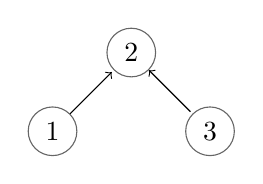
\begin{tikzpicture}[shorten >=1pt,->]
	\tikzstyle{vertex}=[circle, draw=black!60, minimum size=12pt]
	\node[vertex] (G_1) at (-1,-1) {1};
	\node[vertex] (G_2) at (0,0)   {2};
	\node[vertex] (G_3) at (1,-1)  {3};
	\draw [->] (G_1) -- (G_2);
	\draw [<-] (G_2) -- (G_3);
	\end{tikzpicture}
\end{center}
\caption{A graph containing a collider}
\end{figure}

	
\subsection{D-Separation}

If every path between nodes $ X $ and $ Y $ traverses a collider, nodes $ X $ and $ Y $ are unconditionally d-separated or d-separated conditioned on the empty set  ~\parencite{pearl2003causality}. Two unconditionally d-separated nodes in a causal network are considered to be independent ~\parencite{pearl2009}. These concepts are illustrated in Figures 2.4 and 2.5.
\begin{figure}[h]
\begin{center}
	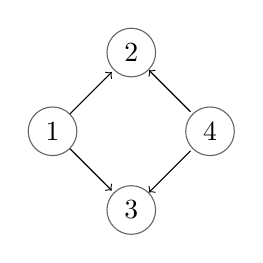
\begin{tikzpicture}[shorten >=1pt,->]
	\tikzstyle{vertex}=[circle, draw=black!60, minimum size=12pt]
	\node[vertex] (G_1) at (-1,-1) {1};
	\node[vertex] (G_2) at (0,0)   {2};
	\node[vertex] (G_3) at (0,-2)  {3};
	\node[vertex] (G_4) at (1,-1)  {4};
	\draw [->] (G_1) -- (G_2);
	\draw [<-] (G_2) -- (G_4);
	\draw [->] (G_1) -- (G_3);
	\draw [<-] (G_3) -- (G_4);
	\end{tikzpicture}
\end{center}
\caption{A DAG in which nodes 1 and 4 are D-Separated}
\end{figure}

\begin{figure}[h]
\begin{center}
	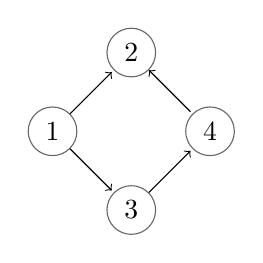
\begin{tikzpicture}[shorten >=1pt,->]
	\tikzstyle{vertex}=[circle, draw=black!60, minimum size=12pt]
	\node[vertex] (G_1) at (4,-1) {1};
	\node[vertex] (G_2) at (5,0)   {2};
	\node[vertex] (G_3) at (5,-2)  {3};
	\node[vertex] (G_4) at (6,-1)  {4};
	\draw [->] (G_1) -- (G_2);
	\draw [<-] (G_2) -- (G_4);
	\draw [->] (G_1) -- (G_3);
	\draw [->] (G_3) -- (G_4);
	\end{tikzpicture}
\end{center}

\caption{A DAG in which nodes 1 and 4 are not D-Separated}
\end{figure}


Two nodes X and Y are d-separated conditioned on set Z if:
\begin{enumerate}
	\item There exists no unblocked path from $ X $ to $ Y $ that does not traverse any members of $ Z $. ~\parencite{pearl2003causality}
	\item There is no blocked path from $ X $ to Y in which all colliders are members of $ Z $ or have descendants in $ Z $.   ~\parencite{pearl2003causality}
\end{enumerate} 

Causal networks represent conditional independence with d-separation, variables X and Y are conditionally independent on set Z if nodes X and Y are d-separated conditioned on nodes in set Z ~\parencite{verma1990causal}.

\section{Faithfulness}


By testing for d-separation of variables X and Y given conditioning set Z on a graph we can see if $X \independent Y | Z$  ~\parencite{pearl2009}. However, the reverse is only true if the distribution is faithful to the graph. That is, if a distribution is faithful to a graph then all independence relationships in the distribution are represented on the graph and only these relationships are present  ~\parencite{scheines1997introduction}. Assuming faithfulness allows the topology of a graph to be learned by testing pairs of variables for independence given various conditioning sets.

\section{Discriminating paths}
For the FCI and RFCI algorithms the notion of discriminating paths is needed. A discriminating path is shown in Figure 2.6. A path $\pi$ = (A, .., X,Y,Z) is a discriminating path for Y if:

\begin{enumerate}
	\item $\pi$ must include at least 3 edges
	\item Y is a non-endpoint on $\pi$ and is adjacent to Z on $\pi$.
	\item A is not adjacent to Z and every other node is a collider on $\pi$ and a parent of Z. ~\parencite{colombo2012learning} 
\end{enumerate}

\begin{figure}[h]
\begin{center}
	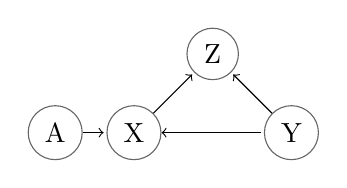
\begin{tikzpicture}[shorten >=1pt,->]
	\tikzstyle{vertex}=[circle, draw=black!60, minimum size=12pt]
	\node[vertex] (G_1) at (0,0) {A};
	\node[vertex] (G_2) at (1,0)   {X};
	\node[vertex] (G_3) at (3,0)  {Y};
	\node[vertex] (G_4) at (2,1)  {Z};
	\draw [->] (G_1) -- (G_2);
	\draw [<-] (G_2) -- (G_3);
	\draw [->] (G_2) -- (G_4);
	\draw [->] (G_3) -- (G_4);
	\end{tikzpicture}
\end{center}


\caption{$A-X-Y-Z$ is a discriminating path on $ Y $}
\end{figure}

\section{Possible D-Separation Set}
The FCI algorithm must also find the possible-d-separation set for every node on the graph. This set consists of all nodes which could be d-separated based on some conditioning set. For a particular node ($ X $) in a graph this set consists of all nodes ($ Y $) for which there exists a path from $ X $ to $ Y $ for which every triple $\langle A,B,C \rangle$ is a triangle or the node $ B $ in the triple is a collider on the path  ~\parencite{colombo2012learning2}.


\section{Tests for Independence}
When trying to find causal relations between variables, tests for independence and conditional independence must be performed. These tests allow us to find dependence between variables and also find out if the dependence between two variables is actually caused by other variables.

One such test is the $\chi^2$ test, this test gives a measure of an observed distribution being equal to an expected distribution.

If the variables $X$ and $Y$ are independent then $p(X,Y) = p(X)p(Y)$. In this case $p(X,Y)$ is the observed distribution an $p(X)p(Y)$ is the expected distribution. Both of these distributions can be estimated from data. The $\chi^2$ test can then be used to find the probability that they are equal ~\parencite{Pearson}.

To estimate $p(X,Y)$ the counts of all pairs of values taken by the variables can be found. They can then divided by the count of all data points. These counts can be stored in a table with the values of $X$ as columns, values of $Y$ as rows (or visa versa) and entries as observed counts, for ease of access. This type of table is known as a contingency table.

\begin{table}[h!]
	\centering
	\begin{tabular}{c|c c c c c c c}
		X & 1 & 1 & 0 & 1 & 0 & 1 & 1\\ \hline
		Y & 0 & 1 & 1 & 1 & 0 & 1 & 0\\
	\end{tabular}
\\
	\begin{tabular}{c|c|cc|}
		\multicolumn{2}{c}{}& \multicolumn{2}{c}{X} \\ \cline{3-4}
		\multicolumn{2}{c|}{} & 0 & 1 \\ \cline{2-4}
		\multirow{2}{*}{Y} & 0 & 1 & 2\\
		& 1 & 1 & 3 \\
		\cline{2-4} 
	\end{tabular}
\caption{Example Contingency Table For Two Variables}
\end{table}

To estimate the distribution $p(X)$, the count of points in which $X$ takes a value over the total number of points for all values of $X$. The counts can be found with the sum of the columns of the contingency table. The same can be done for $p(Y)$ with the rows of the table.\\

The $\chi^2$ statistic can then be calculated with:

\begin{center}
	$\chi^2 = \sum\frac{(p(X)p(Y)-p(X,Y))^2}{p(X)p(Y)}$
\end{center}

The $\chi^2$ value can then be passed to a cumulative density function and a p-value returned. The function used is dependent upon the degrees of freedom. The degrees of freedom are equal to the $(no. rows -1)*(no. columns -1)$ of the contingency table. The p-value represents the confidence that the two variables are not dependent.

The test is similar for conditional independence. The $\chi^2$ statistic now depends on conditional distributions. If $X \independent Y | Z$ $p(X,Y|Z) = p(X|Z)p(Y|Z)$. Therefore:

\begin{center}
	$\chi^2 = \sum\frac{(p(X|Z)p(Y|Z)-p(X,Y|Z))^2}{p(X|Z)p(Y|Z)}$
\end{center}

These values can all be found by calculating a contingency table for $X,Y $ and $ Z$. for all values of the variables.

This statistic can then be used in the same way as before to calculate a p-value. However, the degrees of freedom are multiplied by the number of possible values of $Z$. 

\section{Algorithms For Learning Causal Networks}
\subsection{Constraint Based Methods}
There have been a number of algorithms developed to learn graphical causal representations from data. This project aims to implement up to three constraint based algorithms: The PC algorithm ~\parencite{spirtes1991algorithm}, the Fast Causal Inference (FCI) algorithm ~\parencite{colombo2012learning}, and the Really Fast Causal Inference (RFCI) algorithm ~\parencite{colombo2012learning}.

Rather than learning an individual DAG the PC algorithm learns a set of DAGs which could represent the causal relationships found in the data. In cases where the direction of an edge is unclear no direction is specified. The output of the algorithm is a partially directed acyclic graph which represents the set DAGs with all possible orientations of undirected edges ~\parencite{spirtes1991algorithm}.

The FCI and RFCI algorithms learn partial ancestral graphs (PAGs) which represent Markov equivalence class of MAGs that fit the data  ~\parencite{colombo2012learning}. Unlike in the PC algorithm if the direction of an edge can not be determined it is assumed that there is some set of latent variables influencing the nodes being tested. Each end of an edge can be one of three things in a PAG, an arrow in every MAG ($>$), a tail in every MAG ($-$) or to represent the possibility of latent variables having a causal relationship with an observed variable ($o$), ends of an edge denoted by $*$ can be any of the specified types. This allows for a richer display of information than a partial DAG ~\parencite{colombo2012learning}.

The PAG generated by the FCI algorithm is considered to be less informative than the PAG generated by the RFCI algorithm. This is because the FCI algorithm performs more tests than the RFCI algorithm and applies more constraints. These tests give us more confidence in the presence and the orientation of edges however this comes at the cost of speed ~\parencite{colombo2012learning}.

\subsection{Score Based Methods}
The above algorithms are all constraint based. There is another class of algorithm which are score based. Rather than finding graphs using the rules that define the networks, score based methods search through many graphs. Each graph is assigned a score and the graph which either maximises or minimises the score is chosen.

An example of a scored based method is the graphical lasso algorithm. 

\section{Computing a skeleton}
All three algorithms begin by calculating the skeleton of the graph. The skeleton consists of the edges that are present in the partial DAG or PAG however all edges are undirected. The separation set of two variables ($sepSet(x,y)$) contains the smallest set of variables that the pair are conditionally independent on. When calculating the skeleton the separation set of each pair of variables is also recorded as it is needed to orient the edges of the graph ~\parencite{colombo2012learning, spirtes1991algorithm}.

The skeleton is calculated using a series of conditional independence tests. These conditional independence tests are dependent on the type of input data, therefore conditional independence tests should be defined independently of the algorithm. The conditional independence tests must be able to determine if two variables are independent conditioned on some set of other variables from data ~\parencite{spirtes1991algorithm}.

To begin the skeleton estimation the fully connected undirected graph of all variables is constructed and then conditional independence tests are performed to determine which edges to remove and the separation set of removed edges.

Adjacent pairs of variables are tested for independence conditioned upon a disjoint set of variables adjacent to one of them. The size of these sets starts at 0 but is incremented after all adjacent pairs have been tested. This repeats until there are not enough adjacent variables to fill the conditioning set.\\

The edges which have not been removed by this process form the skeleton of the graph which is needed for the PC, FCI and RFCI algorithms along with the separation sets of removed edges  ~\parencite{spirtes1991algorithm, colombo2012learning}.


\begin{algorithm}[H]
	\DontPrintSemicolon

	\KwIn{Data, Independence Test}
	\KwResult{Estimated Skeleton: $G$, Separating Set of each Variable: $sepSet$}
	\Begin{
	$k = 0$\;
	$N =$ list of variables which make up the data\;
	$G= $ fully connected undirected graph with nodes N\;
	\While{There is some $S \subseteq  adj(X,G) \setminus Y$ and $|S| = k$ for some $X \in N, Y \in adj(X,G) $}{
		\For{$X \in N$}{
			\For{$Y \in adj(X,G)$}{
				\For{$S \subseteq adj(X,G)\setminus Y$ where $|S| = k$}{
					\If{$X \independent Y | S$}{
						remove edge $X-Y$ from G\;
						$Sepset(X,Y) = S$\;
						$Sepset(Y,X) = S$\;
					}
				}
				
			}
		}
	$k += 1$\;
	}
Return $G, sepSet$\;
}
\caption{Algorithm to Estimate Skeleton of Causal Network ~\parencite{spirtes1991algorithm}}
\end{algorithm}
\section{The PC Algorithm}
After generating the skeleton and separation sets of pairs of nodes, the PC algorithm attempts to orient the undirected edges of the graph ~\parencite{spirtes1991algorithm}.

It begins by searching for colliders. For each unshielded triple  $ \langle A, B, C \rangle $, orient the edges $  A-B-C $ to $A\rightarrow B \leftarrow C$ if $ B $ is not in the separation set of the pair $ (A,C) $~\parencite{spirtes1991algorithm}. This can lead to some colliders being overwritten by other colliders which share an edge making this part of the algorithm order dependent.

Once colliders are specified other edges can be oriented. This is done by repeating two steps until no more edges can be given a direction. The process of edge orientation is described in Algorithm 2.\\


\begin{algorithm}[H]
	\DontPrintSemicolon
	
	\KwIn{Skeleton of Causal Network, Separation sets of variables}
	\KwResult{Partial Directed Acyclic Graph}
	\Begin{
	$ 	G = $ Skeleton\;
	$ 	N = $ nodes of G\;
	\For{$i,j,k \in N$}{
	\If{$k \notin adj(i,G)$ and $ j \notin sepSet(i,k)$}{
	orient $i-j-k$ as $i \rightarrow j \leftarrow k$\;
	}	
	}
	\While{No more edges can be oriented}{
	\For{$i,j,k \in N$}{
	\If{ $ k \notin adj(i,G)$}{
	orient $ i\rightarrow j-k $ as $ i\rightarrow j \rightarrow k $\;
	}
	\If{There is a directed path from $i$ to $j$ in $G$}{
	orient $ i-j $ as $ i\rightarrow j$\;
	}
	}
	}
	Return $G$\;
	}
	
	\caption{PC Algorithm to Orient Edges ~\parencite{spirtes1991algorithm}}
\end{algorithm}

\section{The FCI algorithm}

The FCI algorithm starts in the same way as the PC algorithm using exactly the process of conditional independence tests to estimate a skeleton of the final graph. The skeleton is then converted to a PAG by setting all edges to $\circ-\circ$. It orients colliders in the same way, however instead of having to overwrite edges bidirectional edges can be created by overlapping colliders ~\parencite{colombo2012learning2}.

Next, the final skeleton of the graph is obtained from the initial skeleton G . To do this The possible-d-separation set (PossibleDSeps) of every variable must be found in $ G $. These sets are not updated when edges are removed so the order of testing does not affect the outcome. All adjacent variables ($X,Y$) are then tested for conditional independence, conditioned on every subset of each of the PossibleDSeps. If the test finds conditional independence the edge $X,Y$ is removed and the conditioning set recorded as a separation set ~\parencite{colombo2012learning2}. 

Next the colliders must be reoriented. This is done in the same way as earlier.

Once the final skeleton has been estimated, A series of orientation rules can be performed repeatedly until no more orientations are possible. These rules where originally described in ~\parencite{spirtes2001anytime}. However these rules did not fully orient the $-$ tags of the graph ~\parencite{ZHANG20081873}. 10 rules were found in ~\parencite{ZHANG20081873} which allow full orientation of the graph ~\parencite{colombo2012learning}. The complete set of rules is used in the R implementation and will also be used in the Python implementation ~\parencite{kalisch_hauser_maechler}.


\begin{algorithm}[H]
	\DontPrintSemicolon
	
	\KwIn{Skeleton of Causal Network: $G$, Separation sets of variables: $sepSet$}
	\KwResult{Partial Ancestral Graph}
	\Begin{
		$ 	N = $ nodes of $G$\;
		Set all edges of $G$ to $\circ-\circ$\;
		\For{$i,j,k \in N$}{
			\If{$k \notin adj(i,G)$ and $ j \notin sepSet(i,k)$}{
				orient $i *-\circ j \circ-* k$ as $i \circ\rightarrow j \leftarrow \circ k$\;
			}	
		}	
		\For{$i \in N$}{
			\For{$j \in adj(i,G)$}{
				\For{$T \subseteq PossibleDSeps(i,G) \ i$}{
					\If{$i \independent j| T$}{
						remove edge $i*-*j$ from $G$\;
						$sepSet(i,j) = T$\;
						$sepSet(j,i) = T$\;
					}
				}	
			}
		}
		Set all edges of $G$ to $\circ-\circ$\;
		\For{$i,j,k \in N$}{
			\If{$k \notin adj(i,G)$ and $ j \notin sepSet(i,k)$}{
				orient $i *-\circ j \circ-* k$ as $i \circ\rightarrow j \leftarrow \circ k$\;
			}	
		}
		\While{No more edges can be oriented}{
			Apply $R1-R10$ from ~\parencite{ZHANG20081873}
		}
	Return $G, sepSet$\;
	}
	
	\caption{FCI Algorithm to Orient Edges ~\parencite{colombo2012learning2}}
\end{algorithm}


\section{The RFCI Algorithm}
Like the other two algorithms the RFCI begins by estimating the skeleton of the final graph. Next a list of all unshielded triples must be found. The skeleton, separation set and list of triples are fed to Algorithm 4.

Algorithm 4 orients V-structures and updates the separation set. The updated graph is then fed to 
Algorithm 5 to orient the graph fully.

Algorithm 5 uses many of the rules used in Algorithm 3 to orient edges on the graph. It also utilises Algorithm 4 to update the skeleton of the graph as edges are oriented ~\parencite{colombo2012learning}.

\begin{algorithm}[H]
	\DontPrintSemicolon
	
	\KwIn{Skeleton of Causal Network: $G$, Separation sets of variables: $sepSet$, List of unshielded triples: $M$}
	\KwResult{Partial Ancestral Graph}
	\Begin{
		$ 	N = $ nodes of $G$\;
		$ 	L = $ empty list\;
		\While{$M$ is non-empty}{
			choose $\langle i,j,k \rangle$ from $M$\; 
			$T = sepSet(i,k) \ j$\;
			\If{$i \independent j | T$ and $k \independent j | T$}{
				add $\langle i,j,k \rangle$ to $L$
			}
			\Else{
				\For{$r \in {i,j}$}{
					\If{$r \independent j | T$ }{
						Find the minimal separating set $Y \subseteq T$ for $r$ and $j$\;
						$sepSet(r,j) = Y$\;
						$sepSet(j,r) = Y$\;
						add all triples $\langle r,*,j \rangle$ to $M$\;
						Remove all triples containing $r$ and $j$ and either $r$ or $j$ in the middle from $M$ and $L$\;
						Remove $r*-*j$ from $G$\;}
					}
				}
			Remove $\langle i,j,k \rangle$ from $G$\;
			}
			\For{ $\langle i,j,k \rangle \in L$ }{
				\If{$j \notin sepSet(i,k)$}{
					Orient $x*-\circ j \circ - * k$ as $x*-\rightarrow j \leftarrow - * k$}}
				Return $G, sepSet$\;
		}
	\caption{RFCI Algorithm to Orient V-Structures ~\parencite{colombo2012learning2}}
\end{algorithm}

\begin{algorithm}
	\DontPrintSemicolon
	
	\KwIn{Partially oriented Causal Network: $G$, Separation sets of variables: $sepSet$}
	\KwResult{Partial Ancestral Graph}
	\Begin{
		$ 	G = $ network\;
		$ 	N = $ nodes of $G$\;
		\While{no more edges can be oriented}{
			orient as many edges of $G$ as possible using $R1-R3$ from ~\parencite{ZHANG20081873}\;
			\For{$l,j,k \in N$ where $l,j,k is a triangle$}{
				\While{Edges $j\circ - * k, i\leftarrow * j, l\rightarrow k$ exist}{
					Find shortest discriminating paths for $l,j and k$\;
					\If{One of theses paths $\pi$ is between $k$ and $i$}{
						\For{adjacent nodes $r$ and $q \in \pi$}{
							$l = -1$/;
							\While{$|sepSet(i,k) \setminus \{r,q\}| >= l$}{
								$l++$\;
								\For{$ Y \subseteq sepSet(i,k) \setminus \{r,q\}$, where $|Y| = l$}{
									\If{$r \independent q | Y$}{
										$sepSet(r,q) = Y$\;
										$sepSet(q,r) = Y$\;
										Create list M of all triples $\rangle r, *, q \langle$ which form a triangle in $G$\;
										Remove edge $r*-*q$ from G\;
										Run Algorithm 4 with $C, sepSet$ and $M$ as input\;
									}
								}
							}
						}
						\If{All edges in $\pi$ are present in $G$}{
							\If{$j \in sepSet(i,k)$}{
								Orient $j \circ - * k$ as $ j \rightarrow k$
							}
							\Else{
								Orient $l \leftarrow j \circ - * k$ as $l \leftrightarrow j \leftrightarrow k$
							}
						
						}
					} 
				}
			}
			Orient as many edges as possible using $R5-R10$ from ~\parencite{ZHANG20081873}
		}
	Return $G, sepSet$\;
	}
	\caption{RFCI Algorithm to Orient Remaining Edges ~\parencite{colombo2012learning2}}
\end{algorithm}

\chapter{Design}

\section{Methodology}
When designing software there are a number of approaches that can be taken. Most of these approaches break development down into a number of different phases and describe the order in which they should be completed.

Most methodologies were designed for teams of engineers, as this project was completed by one individual many components of the methodologies are redundant. However there are some principles and techniques which can be utilised by an individual developer and aid in the organisation of a project.

\subsection{Waterfall}
The waterfall methodology is a linear approach to development. The project is broken down into stages such as design, implementation and testing. Each stage of development is completed sequentially. This means that once a stage is completed there is no need to return to it and the development process flows in one direction like a a waterfall \parencite{royce1987managing}.

The waterfall approach is good because the whole project is rigorously planned and documented before coding begins. This allows major difficulties in projects to be considered and accounted for. It also allows projects to be easily passed between developers as a new developer can look at the plan of the project. In less linear approaches there may be plans for future parts of software which are not documented and could be lost by the time of implementation.

The downfall of the waterfall approach comes when a project is not a fixed size or there is a a change in requirements, there is no stage in which plans can be modified as that would involve going backwards in development. This makes the project hard to modify once certain stages, such as design, have been completed.


\subsection{Agile}
The agile approach consists of a set of principles which focus on iterative development ~\parencite{beck2001agile}. Deliverables, or functioning pieces of software, are identified and designed individually, there is also a much greater focus on executable code than documentation when compared with waterfall.

Many parts of the agile methodology are not needed in this project such as ways to enable cooperation between developers as this is a solo project.

The most important part of agile is its ability to deal with changing scope throughout the project. Since testing is done at each stage it will allow the project to be easily shortened or extended based on time constraints, as after every sprint a working piece of software has been developed. Therefore so long as each sprint is completed the project will have produced working code. In waterfall this may not be the case.

\subsection{Spiral}
The spiral model for software development is a risk driven process. The spiral method can contain aspects from the other processes ~\parencite{boehm1988spiral}. The actions taken and the amount of work done on areas of the project are determined by what would minimize risk.

Risk can be a number of things. In an industrial setting risk could be how spending more time on a product and delaying its release would affect its sales figures. In a team project, risks could consist of members of the team being unable to work on software unexpectedly because of illness. In essence, risk is anything that would be detrimental to the stakeholders in the project.

Spiral development also requires risks to be assessed at every stage of development. This would increase the work load specifically in agile as risks would need to be identified at every iteration. This would lead to a lot of repeated work that could be better spent on development or testing.  
\subsection{Chosen Approach}

The chosen approach for this project was agile. The reduced amount of documentation increased development speed. Agile development also allows the scope of the project to change over time. This allowed the scope of the project to start off small and increase in size as time allowed it.

For example, once the PC algorithm had been implemented, if time allowed, the project could easily be extended to include the FCI algorithm.

The spiral approach will mostly not be used for this project as it will lead to an unnecessary increase in work for a relatively low risk project. The project also has a fairly logical order of implementation so using risk minimization to determine what to implement will not be necessary. However the choice of the agile methodology due to the risk of change in scope could be considered an application of the spiral method.

Within the Agile methodology there are a number of popular frameworks. However, these methods are designed for teams of software engineers with clients. Since this is a solo project without a client many parts of these frameworks will not be applicable. Therefore, the applicable parts of various frameworks were chosen and compiled into a framework that was specific to this project.

\section{Sprints}
Sprints are sections of development defined by deliverables, sprints are an aspect of the SCRUM framework ~\parencite{schwaber1997scrum}. They outline the tasks required to be completed to develop a deliverable and the time frame needed. The time frame for these sprints was substantially longer than it would be in an industrial setting, this is due to project only being worked on part time by a single individual meaning more time would be needed to create reasonable deliverables.

When a sprint is completed, the scope of the project and the requirements can be updated and modified if needed. For this project there were four main deliverables implemented and four sprints to implement them.

The first sprint consisted of implementing the $\chi ^2$ conditional independence test. This test was needed before anything else could be properly implemented.

Next, the skeleton learning software was written. The skeleton is needed for all algorithms in this project so is the next logical step from the independence test.

Then the PC algorithm was fully implemented, this algorithm was the simplest of the 3 so made sense to start with. Starting with the easiest algorithm gave me experience using networkx and the other libraries being used which was useful when implementing more complex algorithms.

Finally, the FCI algorithm was implemented. This was more complex than the PC algorithm, however the experience with the library in previous sprints gave good insight into it's implementation.

If the project were to continue the next sprint would probably consist of implementing the RFCI algorithm which would easily follow on from the FCI implementation.

\section{Requirements}
Requirements for the project were elicited at the beginning of a sprint. In each sprint a particular deliverable was chosen and the requirements of that deliverable were found. Requirements were found by considering how the software would be used. This is an agile approach to requirement elicitation.

\subsection{Epics}
Epics describe a very high level interaction between a user and the software. They describe the general functionality of a deliverable without discussing the details of implementation. Epics were the first stage of requirement elicitation as they capture the functionality that the requirements must capture ~\parencite{cohn2004user}. Epics can be found in Appendix A.2.

\subsection{User Stories}
Each epic is then broken down into user stories. The stories describe what a user must be able to do with the software during an epic. They are fairly low level and form a set of required functionality of the software ~\parencite{cohn2004user}. User Stories can be found in Appendix A.3.

Users stories can be used as requirements as for a deliverable to fill the role described in a user story it must be functional. So long as the user stories are complete then software implemented based on them will be too.

\subsection{Tasks}
From the stories tasks can be formed. These tasks describe what exactly must be done to fulfil the requirements. Each sprint had a number of associated tasks. The tasks were small and each task could be verified through testing. Tasks can be found in Appendix A.3. 

\section{Architecture}
Only the architecture for a particular deliverable was designed in each sprint. This meant that the architecture grew over time. Considerations for general extensibility of the software needed to be made in the design phase to ease design and implementation during later sprints.

A class diagram was produced, this specified the relationships between classes, such as inheritance and which classes would uses instantiations of the other classes.  The functionality of each class. This diagram evolved throughout the project as various sprints were completed.

The class diagram (see Appendix A.1) for this software was fairly straightforward. This is because the algorithms did not require many classes to be interacting with one another. Each algorithm runs in a single thread and user interaction is minimal. This resulted in a small number of classes keeping the project easy to understand for the purpose of maintenance and future development.
 
\subsection{Unit Testing}
Test driven development (TDD) was one of the main features of the Extreme Programming development framework used  ~\parencite{janzen2005test}. When using TDD, tests were created before the actual software was written. This ensures that all software that is produced functions correctly. It also ensures that any refactoring performed would not compromise the functionality of software. Changing one piece of code in this scenario affected another piece of code that was using it would be very apparent in TDD, whereas this could be missed in other forms of development.

All software was tested using the Python unittest framework. In this framework, list of tests can be compiled into test cases and cases compiled into a test suite. Cases test an individual feature of software, so can be run individually when a feature is being developed or maintained. Test Suites can then test the software as a whole.

\section{Documentation}
All software written was thoroughly documented. Every class, method and function was given an attached doc string detailing its functionality and use.

NumPy style documentation was used ~\parencite{Numpy}. An example is shown in Figure 3.1. This style was chosen because it gives a useful summary of the functionality of a piece of code. It also allows other developers to easily use the code by showing exactly what arguments are taken and exactly what will be returned by a function.

\begin{figure}
\textit{ '''''' A  function to build the set of conditioning sets to be for variables x and y
	on graph G of a certain size when generating a skeleton}

\textit{Parameters\\
	$ 	---------- $\\
	X : str, \\
	One variable being tested for independence\\ 
	Y : str\\
	The other variable being tested for independence\\
	graph : float, optional\\
	The minimum p-value returned by the independence test\\
	for the data to be considered independent\\
	size: int\\
	the size of each conditioning set to be returned\\
	Returns\\
	$ ------- $\\
	str[][]\\
	a list of conditioning sets to be tested\\}
''''''\\
\caption{Numpy Style docstring} 
\end{figure}

Inline comments were also used to clarify areas of code within methods or functions. These comments can allow a developer to quickly and easily understand the code for the purposes of extension or maintenance. They were not as strict in format as the documentation and were mainly used to clarify the code below them.

\section{Tools}
A number of existing tools were used throughout the project to aid in development. 

\subsection{Version Control}
An important part of software development is Version Control (VC). VC allows changes to be made to software without risk of losing previous iterations. At any point software can be reverted to a previous version if needed. VC also helps with agile development as deliverables can be easily identified in a VC system.

Git is a one such VC system. Git was chosen mainly because GitHub provides free repositories which can be used to store code. This makes code accessible from anywhere and greatly reduces the risk of it being lost. GitHub also allows distribution to other developers around the world making the project easily accessible.

\subsection{Python Libraries}
Various external Python libraries were used to facilitate development. They reduced the amount of code that needed to be written increasing development speed and ease.

Pandas is a library containing Data Frames which allow easy manipulation of data. Data Frames store a number of observations of a particular set of variables making them perfect for this application ~\parencite{pandas}. There is also a built in method to calculate a contingency table of the data, this is very useful in the $\chi^2$ test of independence.

NetworkX is a library used for the creation and manipulation of graphs ~\parencite{networkx}, the Graph and Digraph were used and extended to handle various graphs used in the algorithms. The built in functionality of the graphs helped with the implementation of the PDAG and PAG classes. NetworkX also has functions for finding paths in graphs, this was used many times in the various edge orientation rules of the algorithms.

A function from the Scipy statistics library ~\parencite{scipy} was used to in the $\chi^2$ test to calculate the $\chi^2$ statistic and p-value from lists of observed and expected values.

Finally, Numpy arrays used to store the adjacency matrices of graphs. Numpy allows efficient computation with arrays and is used by many other libraries, including pandas. ~\parencite{numpy}  

\section{Refactoring}
Refactoring is a very important part of the agile framework and allows a developer to apply newly gained knowledge to old code. Refactoring consists of rewriting functioning code to improve it.

This improvement could be one of many things. Obvious things like speed and memory consumption may be optimised. However, refactoring can also aid in making code more readable or using a new library that is better suited to the task.

Refactoring may however fail and render previously functional code non-functional. However, this is easily mitigated by unit testing and version control. Unit testing allows a developer to see whether code that has been refactored still functions in the same way as old code, tests will fail if refactoring has been unsuccessful. In the case where refactoring fails a developer can either attempt to identify the problematic area of code and repair/replace it or use the version control system to easily roll back to an existing functional version of the software. These two systems hugely mitigate the risks of refactoring.

\chapter{Implementation}

\section{Independence Test}
The first sprint consisted of implementing the  $\chi^2$ tests for independence and conditional independence. This test is needed for skeleton estimation, which is used in the PC, FCI, and RFCI algorithms so is the logical starting point of the project. This test will only work on discrete data dan relatively large datasets however other tests could be substituted for learning causal networks from other types of data.

Pandas Data Frames were chosen to store data throughout the algorithm as they provide easy indexing, labelling and many useful functions. For example, the crosstab function was used to find contingency tables for the $\chi^2$ test.

A function prepare\_data was implemented to read data from a file into a data frame for processing. This function is a method of all algorithm classes in the project.

The unconditional independence test was fairly straightforward to implement as it only consisted of computing the contingency tables and then comparing the values in the tables to the sums of the rows and columns in the tables.

In the conditional case the conditioning set was combined into a single variable through concatenation of each variable and every data point in the conditioning set. Next a contingency table across the three variables was needed. The distributions needed were then calculated from the contingency table and a p-value calculated.

In some cases $p(X,Y|Z) = 0$, this would cause a divide by zero error. This is due to the $\chi^2$ test not being suitable for small datasets. Other tests should be used in these cases, like Fishers exact test. As the main purpose of the project was to implement the algorithms rather than independence tests, and the test can easily be substituted, this implementation of the $\chi^2$ test was slightly altered to allow the algorithms to be tested. If  $p(X,Y|Z) = 0$ it was replaced with a number arbitrarily close to 0 (0.0.000000000001). This produced the same results as the bnlearn implementation, in the future this should be replaced with an exception and a recommendation to use another independence test.

The scipy chi2 function was then used to calculate the $chi^2$ statistic and p-value which are both returned by the independence test function.
\section{Skeleton}
\subsection{Variables to be Tested}
With this function the skeleton can be found. A fully connected networkx Graph, with the variables as nodes, is generated and then edges between nodes that show conditional independence are removed. 

First unconditional independence tests are performed between each pair of variables. Edges are removed between those that are found to be independent. The conditional tests are based upon variables adjacent to the first variable with the size of this set increasing by one after all possible tests have been performed. The algorithm tests $X \independent Y | Z$ and $Y \independent X | Z$, this may seem inefficient as it appears that tests are being repeated. However, the members of the set $Z$ are dependent on the first variable in the statement. This means that the tests must all be performed.

To find the conditioning sets, the combinations function from the Python library itertools was used to find all subsets of $adj(x,G)\ y$ of a certain size.

\subsection{Separation Sets}
Edge orientation requires the separation set of each pair of variables. This was stored as a dictionary of all pairs of edges and simply updated with a conditioning set if that pair was found to be independent when condition on that set.

Since all of the algorithms learn a skeleton, the function is a method of the GraphLearner class which is the parent class of the other algorithm classes. The function returns a networkx Graph containing the estimated edges of the skeleton and a dictionary containing the separation set of each pair of variables.

\section{PC Edge Orientation}
For the PC algorithm edge orientation is relatively simple. However, the PC algorithm outputs a PDAG which contains a mixture of directed and undirected edges, networkx does not contain a data structure to support this kind of graph so one had to be implemented. This turned out to be fairly trivial, using a directed graph behind the scenes in which undirected edges were represented as bidirectional edge. Since a DAG there cannot contain any bidirectional edges so all bidirectional edges can simply be considered to be undirected.

When orienting edges of a graph, one graph was used to store directed and one used to store undirected. When an edge was directed it was simply transferred from one to the other. Once all edges that can be oriented are oriented, the two graphs are combined into a PDAG.

\subsection{V-Structures}
The first part of edge orientation consists of identifying colliders. This is fairly simple as you simply need to iterate over all triples, test to see whether the triple is unshielded and finally check the separation set.

However, there may be situations in which the order of the v-structures you test affects the final orientation of the graph. There may be two connected v-structures where orienting one will also orient the other but not in the direction described by the constraints.

\begin{figure}[h]
\begin{center}
	
	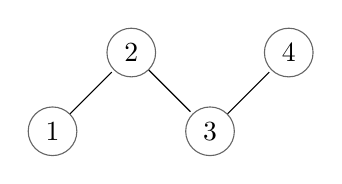
\begin{tikzpicture}[shorten >=1pt,->]
	\tikzstyle{vertex}=[circle, draw=black!60, minimum size=12pt]
	\node[vertex] (G_1) at (-1,-1) {1};
	\node[vertex] (G_2) at (0,0)   {2};
	\node[vertex] (G_3) at (1,-1)  {3};
	\node[vertex] (G_4) at (2,0)  {4};
	\draw [-] (G_1) -- (G_2);
	\draw [-] (G_2) -- (G_3);
	\draw [-] (G_3) -- (G_4);
	\end{tikzpicture}
\end{center}
\caption{A skeleton of a Causal Network}
\end{figure}

\begin{figure}[h]
\begin{center}
	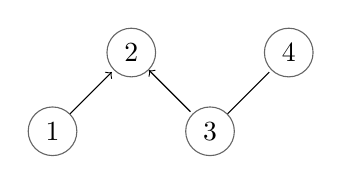
\begin{tikzpicture}[shorten >=1pt,->]
	\tikzstyle{vertex}=[circle, draw=black!60, minimum size=12pt]
	\node[vertex] (G_1) at (-1,-1) {1};
	\node[vertex] (G_2) at (0,0)   {2};
	\node[vertex] (G_3) at (1,-1)  {3};
	\node[vertex] (G_4) at (2,0)  {4};
	\draw [->] (G_1) -- (G_2);
	\draw [<-] (G_2) -- (G_3);
	\draw [-] (G_3) -- (G_4);
	\end{tikzpicture}
	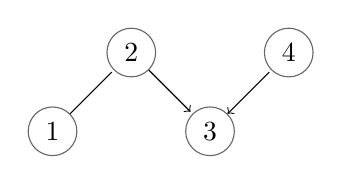
\begin{tikzpicture}[shorten >=1pt,->]
	\tikzstyle{vertex}=[circle, draw=black!60, minimum size=12pt]
	\node[vertex] (G_1) at (-1,-1) {1};
	\node[vertex] (G_2) at (0,0)   {2};
	\node[vertex] (G_3) at (1,-1)  {3};
	\node[vertex] (G_4) at (2,0)  {4};
	\draw [-] (G_1) -- (G_2);
	\draw [->] (G_2) -- (G_3);
	\draw [<-] (G_3) -- (G_4);
	\end{tikzpicture}
\end{center}
\caption{Two potential colliders in a skeleton}
\end{figure}
Figure 4.1 shows two possible orientations of the skeleton in Figure 4.2, depending on which v structure is oriented first, in the first case when we arrive at the triple $\langle 2,3,4 \rangle$ one of two thing can be done. The edge (3-4) can be left undirected or the new structure can override the old one, as shown in Figure 4.3.
\begin{figure}[h]
\begin{center}
	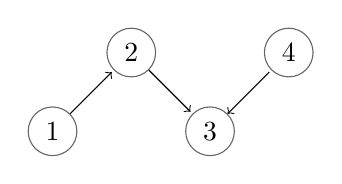
\begin{tikzpicture}[shorten >=1pt,->]
	\tikzstyle{vertex}=[circle, draw=black!60, minimum size=12pt]
	\node[vertex] (G_1) at (-1,-1) {1};
	\node[vertex] (G_2) at (0,0)   {2};
	\node[vertex] (G_3) at (1,-1)  {3};
	\node[vertex] (G_4) at (2,0)  {4};
	\draw [->] (G_1) -- (G_2);
	\draw [->] (G_2) -- (G_3);
	\draw [<-] (G_3) -- (G_4);
	\end{tikzpicture}
\end{center}
\caption{A potential orientation of the skeleton in Figure 4.1 containing colliders from Figure 4.2}
\end{figure}
In the pre-existing R implementation the second approach of overwriting edges was taken so the same was done in the Python implementation for consistency ~\parencite{colombo2012learning2}.

Finally the other orientation rules described in the algorithm were followed, these were easy to implement using the networkx graphs. The all\_simple\_paths functions was very useful in the second orientation rule.

\section{FCI Algorithm Edge Orientation}

The FCI algorithm was able to use the same skeleton estimation method. After this the skeleton is converted to a PAG with all circle tags. The collider orientation code was also very similar, however must now operate on a PAG instead of the two graphs from the PC algorithm. After this, code unique to the FCI algorithm must be developed.

First, the final skeleton of the graph must be found. This is done by performing more independence tests, which are conditioned on the possible d-separating sets of the variables. Finding these sets was made easier by a networkx function to find paths between nodes on a graph. For the rest of the algorithm the network is a PAG. 

The data structure used for the PAG was a subclass of the networkx undirected graph. In this graph the direction of an edge was determined by tags stored in a dictionary associated with that edge. This allowed all edge types of a PAG to be stored.

\section{Testing}

To ensure that the implementation behaving as intended all parts were thoroughly tested. The Python unittest module was used to create a test suite covering as many aspects of the algorithm as possible.

\subsection{Independence Test}
For the $\chi^2$ independence test, a sanity check consisting of testing whether a variable was independent of itself was used. Obviously the test will result in a p-value of 0 so was very easy to test. This test was repeated in the case of a conditioning set of size 1 and size 2 to ensure that it did not affect functionality.

Next a pre-existing test from the R bnlearn library was used to find results on real data. This data was tested with the Python implementation and the results compared. Data from the Alarm\_10000 the Asia\_10000 and the Asia\_1000 datasets were used from \parencite{data}. These datasets have been generated from casual networks and are discrete. Many tests with different variables and conditioning sets were performed.

\subsection{Skeleton Estimation}
To test the skeleton estimation the R implementation was used again. However, the R version does not use a chi squared test, a wrapper needed to be written to make it compatible with the bnlearn function. With this, skeletons could be generated from data in the same way in Python and R and the results compared. The separation sets were also recorded and compared.

\subsection{PC Algorithm}
Testing the edge orientation for the PC algorithm first started with small sanity checks. For example the collider orientation was tested on networks with 3 nodes and two edges and simple separation sets.

Finally a skeleton and separation set generated from the alarms data was oriented in both R and Python to test the whole edge orientation process as a whole.

\subsection{FCI Algorithm}
For the FCI algorithm, the first part of the skeleton estimation is the same as in the PC algorithm. However, the final skeleton estimation needs to be tested so comparison testing was done with the R implementation.

Each orientation rule was tested. The rules were tested on graphs which the rule should be applied to and graphs which the rule should not be applied to. The graphs were then tested after rule had been tried to see if the edges had been oriented correctly.

\subsection{Final Structure}
The final implementation consisted of four main components. The $\chi^2$ test for independence, the skeleton estimation, PC algorithm, and FCI algorithm.

\subsection{Independence Test}
The $\chi^2$ test was a stand-alone function that can take a data frame along with the names of variables to be tested and a conditioning set. It returns a the $\chi^2$ statistic and a p-value from the test. The p-value represents the probability that the variables are not dependent conditioned on the conditioning set, if this statistic is high enough the variables can be considered independent.

\subsection{Graph Learners}
Each algorithm is implemented as a class, the base class of all algorithms is the graph learner class. These classes take data and an independence test and learn a graph.

The base class implements the skeleton learning method that all the algorithms use. It can also find and orient colliders on that skeleton. Finally, it has a static method to prepare data, this reads data from a file into a dataframe which can be used by the other methods.

The PC algorithm and the FCI algorithms were implemented as subclasses of the Graph learner and added the other functionality they required.

\subsection{Graphs}  
Two new graph classes were implemented, the PDAG and the PAG. The PDAG is a fairly simple extension of networkx's built in Directed graph class in which undirected edges are merely stored as bidirectional edges, in PDAGs there are no bidirectional edges so there will be no confusions between bidirectional and undirected edges. An example of a PDAG and its underlying representation is shown in Figure 4.4.

This implementation is simple but fairly powerful. Most built in networkx functions will work in a reasonable manner. For example, the has\_edge function will be direction dependent on directed edges but not on undirected edges. Path finding algorithms will also work assuming undirected edges can be traversed in either direction.

\begin{figure}[h]
\begin{center}
	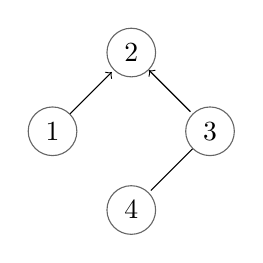
\begin{tikzpicture}[shorten >=1pt,->]
	\tikzstyle{vertex}=[circle, draw=black!60, minimum size=12pt]
	\node[vertex] (G_1) at (-1,-1) {1};
	\node[vertex] (G_2) at (0,0)   {2};
	\node[vertex] (G_3) at (1,-1)  {3};
	\node[vertex] (G_4) at (0,-2)  {4};
	\draw [->] (G_1) -- (G_2);
	\draw [<-] (G_2) -- (G_3);
	\draw [-] (G_3) -- (G_4);
	\end{tikzpicture}
	\quad\quad
	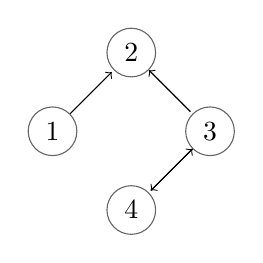
\begin{tikzpicture}[shorten >=1pt,->]
	\tikzstyle{vertex}=[circle, draw=black!60, minimum size=12pt]
	\node[vertex] (G_1) at (-1,-1) {1};
	\node[vertex] (G_2) at (0,0)   {2};
	\node[vertex] (G_3) at (1,-1)  {3};
	\node[vertex] (G_4) at (0,-2)  {4};
	\draw [->] (G_1) -- (G_2);
	\draw [<-] (G_2) -- (G_3);
	\draw [<-] (G_3) -- (G_4);
	\draw [->] (G_3) -- (G_4);
	\end{tikzpicture}
\end{center}
\caption{A PDAG and how it would be represented in the implementation}
\end{figure}
The PAG was more complex to implement due to the increased complexity of the graph. The PAG class is an extension of the undirected graph from networkx. 

All information about the tags, and therefore the directionality of the edges is stored in an attribute associated with particular edge. The attribute is a dictionary with keys being the nodes at each end of the edge and the values being the tag at that end of the edge. An example of a PAG and its underlying representation is shown in Figure 4.5.

This implementation meant that many new methods needed to be added and many existing methods modified. For example, when adding a new edge the tags of the edge needed to be assigned.

\begin{figure}[h]
\begin{center}
	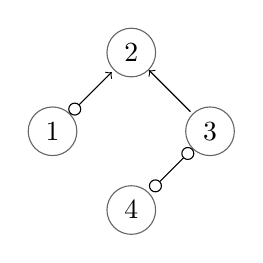
\begin{tikzpicture}[shorten >=1pt,->]
	\tikzstyle{vertex}=[circle, draw=black!60, minimum size=12pt]
	\node[vertex] (G_1) at (-1,-1) {1};
	\node[vertex] (G_2) at (0,0)   {2};
	\node[vertex] (G_3) at (1,-1)  {3};
	\node[vertex] (G_4) at (0,-2)  {4};
	\draw [o->] (G_1) -- (G_2);
	\draw [<-] (G_2) -- (G_3);
	\draw [o-o] (G_3) -- (G_4);
	\end{tikzpicture}
	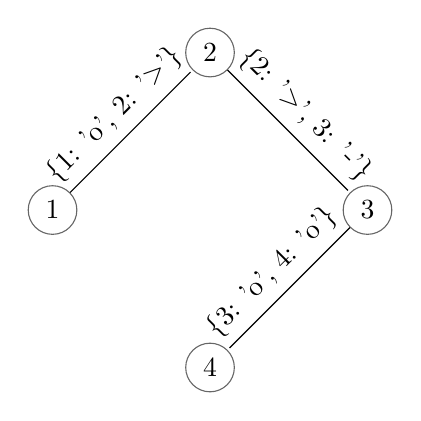
\begin{tikzpicture}[shorten >=1pt,->]
	\tikzstyle{vertex}=[circle, draw=black!60, minimum size=12pt]
	\node[vertex] (G_1) at (-1,-1) {1};
	\node[vertex] (G_2) at (1,1)   {2};
	\node[vertex] (G_3) at (3,-1)  {3};
	\node[vertex] (G_4) at (1,-3)  {4};
	\draw [-] (G_1) -- node[sloped, above]{\{1: 'o', 2: '$>$'\}} (G_2) ;
	\draw [-] (G_2) -- node[sloped, above]{\{2: '$>$', 3: '-'\}} (G_3);
	\draw [-] (G_3) -- node[sloped, above]{\{3: 'o', 4: 'o'\}} (G_4);
	\end{tikzpicture}
\end{center}
\caption{A PAG and how it would be represented in the implementation}
\end{figure}
\section{Usage}
There are currently two main ways to use the Python implementation, as a library and as a command line interface.

The usage of the various objects and data structures is described in the docstring of each class, they can simply be imported and used as part of a wider program.

To use the PC or FCI algorithm, simply run the program from a command line with the path to the data file as the first argument. Optional parameters are available to state if the data is labelled (default False) and what the delineator (default ' ') is. Data should consist of rows of observations and columns of variables, the first row may consist of labels for each column. For example, to use the FCI algorithm on the insurance\_1000 dataset (unlabelled and separated by spaces) simply call:

\textbf{src/fci.py data/insurance\_1000.data False space}

In the main directory of the project. The adjacency matrix will be written to a file called adjmat in the same folder for future usage.
 
\section{Viewing Graphs}
There are a number of options to view a learned graph. Built in functions of the parent classes allow the edges and nodes to be iterated over to see where causal links have been estimated.

\subsection{Adjacency Matrices}
Options to view the graphs as adjacency matrices have also been implemented. In these matrices the rows represent the from node and the columns represent a to node. The order of the rows and columns is the same as the order in which the nodes are iterated over. The matrix is stored as a numpy array so it can be used with efficient numpy methods in the future.

In the PDAG when there is a directed edge from one node to another there is a one in the appropriate position. If there is not a directed edge there is a zero. Directed edges going in both directions between nodes represent an undirected edge.
 
The PAG uses numbers greater than zero to represent the tags on an edge and zeroes to represent the absence of an edge. the '0' tag is represented as a one, the '-' tag as a two and the '>' tag as a three.

These matrices can also be written to files for future use. Each row of the matrix is written as a row values in a row are separated by spaces. The first row of the file consists of the node name of the respective column. The first value of each row of points is the name of the corresponding node.

\chapter{Analysis}
Analysis of this project will mainly consist of comparison to the implementation of the algorithms in R, where possible. It will compare the functionality of the algorithms on data and also the run speed of the code. 

Order dependence of the algorithms, as discussed in ~\parencite{colombo2014order}, was a major issue when it came to this analysis. The nature of the algorithms being implemented mean that multiple valid implementations can produce different results on the same data. There is no correct or standard order for the order dependent parts of the algorithm.n.

In fact, attempting to validate the project by looking at the output of each algorithm makes little sense due to the ambiguity. One set of parameters can have many valid outputs from each algorithm. It make more sense to individually validate each stage in the algorithm in which the graph is modified. Ensuring graphs are only modified under the correct conditions and the modifications that are made are correct. This can be done through unit testing.

To generate the desired values for testing, they can either be generated by the R implementation or generated manually on simple networks.

The functionality of the implementation is hard to quantify. Unlike other projects, this code produce a statistic denoting how well a particular implementation has performed on a particular dataset. Outputs of this algorithm also should not be compared to the actual graphs that generated the data, in an attempt to validate software. This is because the algorithms themselves may incorrectly estimate a graph regardless of the validity of the implementation.

\section{Independence Test}
The $\chi^2$ test for independence was not implemented in the pcalg library in R. Other independence test for discrete data, such as the $G^2$ test, were implemented. Fortunately, the bnlearn library has an implementation of the $\chi^2$ test which can be used for comparison.

The two tests return identical results on variables in the Alarm\_10000, Alarm\_1000, Asia\_1000, the Asia\_10000, and the Insurance\_1000 datasets found in ~\parencite{data}, these comparisons can be found in the unit tests of the project.

\section{Initial Skeleton Generation}
The skeleton generation code has identical functionality as the R implementation. However the R implementation has a non-order dependent mode which is not currently implemented in the Python version. This could be added as an option in the future. Fortunately the order in which tests are done in both versions is the same so as long as the data is provided in the same order they will generate the same results.


\section{PC Algorithm Edge Orientation}
\begin{figure}[h]
\begin{center}
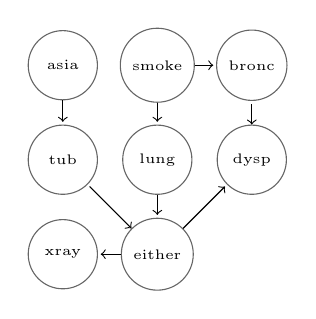
\begin{tikzpicture}[shorten >=1pt,->]
\tikzstyle{vertex}=[circle, draw=black!60, minimum size=25pt, font=\tiny]
\node[vertex] (asia) at (-1.2,1.2) {asia};
\node[vertex] (tub) at (-1.2,0) {tub};
\node[vertex] (smoke) at (0,1.2) {smoke};
\node[vertex] (lung) at (0,0) {lung};
\node[vertex] (bronc) at (1.2,1.2) {bronc};
\node[vertex] (either) at (0,-1.2) {either};
\node[vertex] (xray) at (-1.2,-1.2) {xray};
\node[vertex] (dysp) at (1.2,0) {dysp};
\draw [<-] (dysp) -- (bronc);
\draw [->] (smoke) -- (bronc);
\draw [->] (smoke) -- (lung);
\draw [->] (asia) -- (tub);
\draw [->] (lung) -- (either);
\draw [<-] (either) -- (tub);
\draw [->] (either) -- (xray);
\draw [->] (either) -- (dysp);

\end{tikzpicture}
\end{center}
\caption{The actual network that generated data in the asia\_1000 dataset}
\end{figure}
\begin{figure}[h]
\begin{center}
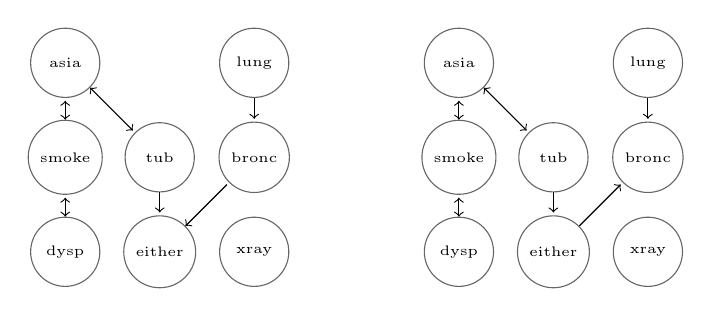
\begin{tikzpicture}[shorten >=1pt,->]
\tikzstyle{vertex}=[circle, draw=black!60, minimum size=25pt, font=\tiny]
\node[vertex] (asia) at (-1.2,1.2) {asia};
\node[vertex] (tub) at (0,0) {tub};
\node[vertex] (smoke) at (-1.2,0) {smoke};
\node[vertex] (lung) at (1.2,1.2) {lung};
\node[vertex] (bronc) at (1.2,0) {bronc};
\node[vertex] (either) at (0,-1.2) {either};
\node[vertex] (xray) at (1.2,-1.2) {xray};
\node[vertex] (dysp) at (-1.2,-1.2) {dysp};
\draw [<->] (dysp) -- (smoke);
\draw [<->] (smoke) -- (asia);
\draw [<->] (asia) -- (tub);
\draw [->] (tub) -- (either);
\draw [<-] (either) -- (bronc);
\draw [->] (lung) -- (bronc);[shorten >=1pt,->]

\node[vertex] (asia) at (3.8,1.2) {asia};
\node[vertex] (tub) at (5,0) {tub};
\node[vertex] (smoke) at (3.8,0) {smoke};
\node[vertex] (lung) at (6.2,1.2) {lung};
\node[vertex] (bronc) at (6.2,0) {bronc};
\node[vertex] (either) at (5,-1.2) {either};
\node[vertex] (xray) at (6.2,-1.2) {xray};
\node[vertex] (dysp) at (3.8,-1.2) {dysp};
\draw [<->] (dysp) -- (smoke);
\draw [<->] (smoke) -- (asia);
\draw [<->] (asia) -- (tub);
\draw [->] (tub) -- (either);
\draw [->] (either) -- (bronc);
\draw [->] (lung) -- (bronc);
\end{tikzpicture}
\end{center}
\caption{The networks estimated by the R (left) and Python (right) implementation from the Asia\_1000 dataset}
\end{figure}

There are some differences in the edge orientation of the different implementations. For example, in the orientation of the Asia\_1000 network, the edge either-bronc is oriented in opposite directions by the two implementations, see Figure 5.2. When tested on other datasets similar results were found, with identical skeletons but edges oriented indifferent directions. 

This difference is due to the order in which the colliders were oriented in the graph. In the R implementation the triple $ \langle lung, bronc, either\rangle$ is oriented before the triple $ \langle tub, either, bronc \rangle $. This causes the edge either-bronc to be overwritten and reoriented. In the Python implementation this is done in the opposite order resulting in a different network.

The algorithm does not specify an order to search for colliders to orient. This leads to different orientations of edges, but this is a problem in the specification of the algorithm rather than the particular implementations. This is a major flaw in all of the algorithms and can have major effects, seeming to imply that the direction of causation changes depending on the order in which the algorithm constrains parts of the network.

This problem has been addressed in ~\parencite{colombo2014order} which discusses a number of modifications to the algorithm to remove the order dependence, these modifications are available in the R implementation. Unfortunately also implementing these order independent methods was not possible due to time constraints.

Because of these differences doing straight comparisons of the two implementations would not show whether or not the python implementation was a correct implementation of the algorithm.

It is instead better to view the output of the implementation and the rules that were applied to produce the output. If all rules were applied at appropriate times and all rules have been confirmed to function correctly through unit testing then the code must be functioning correctly. This was done using unitttests and the code was found to be functioning correctly.

It is worth noting that both estimates are quite different from the actual network which generated the data, see Figure 5.1.

\section{FCI Algorithm Final Skeleton}
The FCI algorithm begins with the same skeleton estimation as the PC algorithm. At this point there is a divergence between the two implementations in the orientation of colliders. The collider orientation in the Python implementation is as ~\parencite{colombo2012learning2} describes, whereas the R implementation uses a non order dependent method (the conservative method) described in ~\parencite{colombo2014order}, producing different results. 

The modified orientation affects the input to the later stages of the algorithm, some of which remove edges from the graph, so could make large differences to the final output. This modification is inconsistent with the R implementation of the PC algorithm which doesn't use this order independent V structure orientation.

This does not result in differences the estimation of the Asia\_1000 graph, however it will affect other graphs and since it is done fairly early on in the algorithm it can have large knock-on affects on the end result.

As the two implementations are actually of slightly different algorithms it does not make sense to compare the whole algorithm across the implementations. Instead, if every component of this part of the algorithm can be proved to function as specified using unit tests then the skeleton estimation can be assumed to work properly.

The R implementation was used to generate tests for the rest of the skeleton learning including the generation of possible d sep sets. This allowed them to be individually tested without the knock on affect of previous steps.

\section{FCI Algorithm Edge Orientation}

Unit testing was used to individually test rule application for edge orientation. The rules were tested on many different graphs, ones which should be modified and ones which shouldn't. This was done for every single orientation step in the algorithm and proved that the orientation rules function correctly.

 
\section{Run Speed}
The cProfiling library was used to collect statistics about the implementation. The library collects the number of times each function is called by the code along with the execution time of the code. This profiling allows the bottle necks of the code to be found and made high priorities or optimisation.

The independence test was the main bottleneck of the algorithms, and was significantly slower than the R implementation. This is because the R implementation actually runs C code behind the scenes, C code tends to run faster than Python and R code ~\parencite{wilbers2009using, wilkinson_2014}.

Calculating the contingency tables was the most expensive part of the independence test (86\% of total runtime of the PC algorithm on the Alarm\_10000 dataset). Currently it uses a built in function from the pandas library. Replacing this function with something faster could make a large difference to the run speed.

However, the independence test in the algorithm is a parameter and thus the current slow test could be wholly replaced by a faster version. This new test could call C code like the R implementation.

The edge orientation also begins to take a large amount of time on datasets with more variables. This is due to the greater number of edges to search through. This search could almost certainly be refined to improve the efficiency of the program.

Overall the implementations were both found to be functional, passing 60 unit tests. In these tests every component of each algorithm was tested in a number of situations.

However there were slight differences when compared the R implementation due to different versions of the algorithms being implemented along with the order dependence issues of the algorithms affecting output.

\chapter{Conclusion}
In conclusion, the project was successful. Two algorithms were implemented which are able to learn causal networks in Python. These implementations provide an easy to use framework and a framework that will also be easy to extend in the future.

\section{Further Work}
The most obvious extension to this project would be to implement the RFCI algorithm described in the literature review. Due to time constraints it was not implemented for this project. However the PAG class implements the majority of functionality needed to implement the RFCI algorithm. The process of implementation would be very similar to the process of implementing the FCI algorithm. It was be reasonable to simply extend the FCIAlg class to take advantage of the existing functionality. The non-order dependent algorithms described in ~\parencite{colombo2014order} could be also be implemented.

Another improvement would be to increase the speed of the conditional independence tests. One approach could be to implement the independence test in C and interface with it using Cython ~\parencite{cython}. C programs can be much faster than those written in Python so there would almost definitely be an improvement ~\parencite{wilbers2009using}.

Other independence tests could also be written. These tests could be for the same kind of data as the $\chi^2$ or it could be a test for other data for example continuous data. The raw data would not even be necessary input to the algorithm, instead some sufficient statistics placed in a pandas data frame could be used if the independence test was able to estimate independence based on these statistics.

\printbibliography
\appendix
\chapter{Appendix}
\section{UML Class Diagram}
\includegraphics[height = 4in]{"./Causal Nets"}\\
\section{Epics}
\begin{tabular}{| l | p{12cm} |}
	\hline	
	ID & Epic \\
	\hline
	1 & A user must be able to learn a Graph, representing causal relationships, from data \\
	\hline
	2 & A user must be able to view a learned graph \\
	\hline
	3 & A user must be able to save a learned graph to a file\\
	\hline
\end{tabular}
\section{User Stories}
\begin{tabular}{| l | l | p{9.5cm} |}
	\hline
	Epic ID & Story ID & Story \\
	\hline
	\multirow{6}{*}{1} & 1.1 & A user must be able to define a custom conditional independence  function\\
	\cline{2-3}
	& 1.2 & A user  must be able to learn a Directed Acyclic Graph using  the PC algorithm \\
	\cline{2-3}
	& 1.3 & A user  must be able to learn a Partial  Ancestral Graph using  the FCI algorithm \\
	\cline{2-3}
	& 1.5 & A user must have access to  predefined conditional independence function \\
	\cline{2-3}
	& 1.6 & A user must be able to estimate the skeleton of a graph \\
	\cline{2-3}
	& 1.7 & A user must be able to read data from a file into an appropriate data structure \\
	\hline
	\multirow{3}{*}{2}
	& 2.1 & A user must have access to a data structure containing edges of the graph \\
	\cline{2-3}
	& 2.2 & A user must be able to tell if an edge is directed or not in a PAG \\
	\cline{2-3}
	& 2.3 & A user must be able to tell how an edge is labelled on a PAG \\
	\hline
	\multirow{4}{*}{3}
	& 3.1 & A user must be able to convert the graph into an adjacency matrix \\
	\cline{2-3}
	& 3.2 & A user must be able to write an adjacency matrix to a file \\
	\cline{2-3}
	& 3.3 & A user must be able to distinguish edge label in the adj matrix of a PAG \\
	\cline{2-3}
	& 3.3 & A user must be able to distinguish whether or not an edge is directed or not  in the adj matrix of a PDAG \\
	\hline
	
\end{tabular}
\section{Sprints and Tasks}
\begin{tabular}{| l |p{9cm}|}
	\hline
	Sprint & Tasks\\
	\hline
	\multirow{3}{*}{Chi Squared Test} & Calculate contingency tables from data \\
	\cline{2-2}
	& Iterate over contingency table to calculate the two distributions \\
	\cline{2-2}
	& Calculate a p-value from the distributions \\
	\cline{2-2}
	\hline
	\multirow{3}{*}{Learn Skeleton} & Implement a base graph learner class\\
	\cline{2-2}
	& 
	Calculate conditioning sets for all pairs of nodes
	 \\
	\cline{2-2}
	& Remove independent edges from graph \\
	\cline{2-2}
	\hline
	\multirow{3}{*}{PC Algorithm} & 
	Implement a PDAG data structure \\
	\cline{2-2}
	& Orient V structures \\
	\cline{2-2}
	& Orient further edges \\
	\cline{2-2}
	\hline
	\multirow{4}{*}{FCI Algorithm} & Implement a PAG data structure \\
	\cline{2-2}
	& Orient V structures \\
	\cline{2-2}
	& Find possible d-sep-sets \\
	\cline{2-2}
	& Implement rules 1-10 to orient edges \\
	\cline{2-2}
	\hline
\end{tabular}

\end{document}